\chapter{Diseño de Investigación}
%http://recipp.ipp.pt/bitstream/10400.22/136/3/KDD-CRISP-SEMMA.pdf
%http://www.oldemarrodriguez.com/yahoo_site_admin/assets/docs/Documento_CRISP-DM.2385037

\section{Introducción}
En un principio el proyecto comienza como parte de una necesidad que surge a la CEI. Dicha necesidad se basa en realizar explotaciones (visualizando los datos según convenga) y reportes sobre la situación actual respecto a otros años, concretamente, los últimos 10 años \footnote{Antes del curso 2007/2008 no existe un sistema de gestión centralizado y por lo tanto no se puede hacer explotaciones}. Véase el Anexo \ref{appendix:C} para más información.

La CEI dispone de un gran número de bases de datos, por lo que obtener información sencilla a través de ellas resulta complejo. Por tanto, se requiere de un sistema de explotación que permita obtener el máximo valor de la información de dichas bases de datos.

Las bases de datos de este sistema de explotación se encuentran en un estado en el que es sencillo poder realizar análisis exploratorios y predictivos (ya que los datos se encuentran limpios y transformados a conveniencia), por tanto, a partir de este estado, se contempla la ampliación y la resolución de las nuevas necesidades de la CEI sobre la planificación de las unidades.

\section{Diseño de la minería de datos}
Una vez que se tiene claro la arquitectura principal del sistema, se establece el camino a seguir a la hora de realizar la investigación. Para ello, se utiliza la metodología CRISP-DM. \citeA{IBMCRISP2012}

La metodología CRISP-DM tiene como objetivo orientar los proyectos de minería de datos. 
\begin{itemize}
	\item Como metodología: incluye descripciones de las fases normales de un proyecto, las tareas necesarias en cada una de las fases y una explicación de las relaciones entre las tareas.
	\item Como modelo de proceso: ofrece un resumen del ciclo vital de la minería de datos.
\end{itemize}

La metodología CRISP-DM establece un proceso genérico para satisfacer los objetivos deseados y contemplar la realización de la vigilancia e inteligencia. Este proceso se divide en distintas etapas básicas. 

\begin{figure*}[h]
\centering
\caption{Fases del ciclo de vida de CRISP-DM. Recuperado de \protect\citeA{IBMCRISP2012}.}
 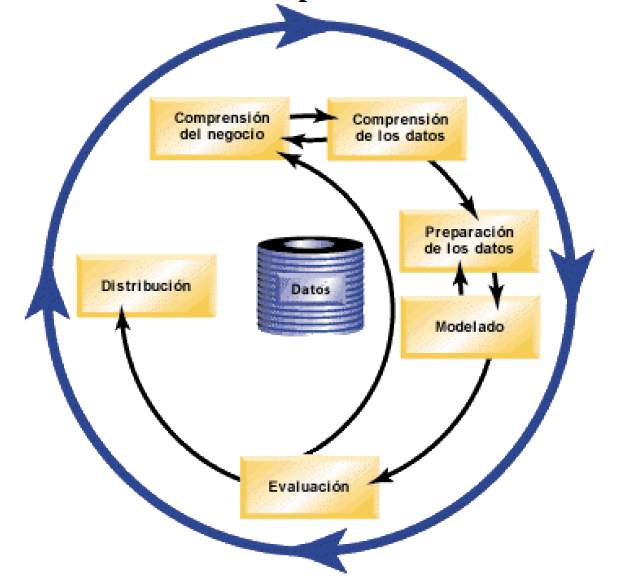
\includegraphics[width=0.6\textwidth]{recursos/CRISPCicloIBM}
\label{fig:CicloCrispDM}
\end{figure*}
\FloatBarrier
El ciclo de vida de CRISP-DM está compuesto de seis fases. La secuencia de estas no es estricta, es más, la mayoría de proyectos avanzan y retroceden entre fases si es necesario. En la figura \ref{fig:CicloCrispDM} se puede observar cada fase:

\begin{enumerate}
	\item \textbf{Comprensión del negocio.} Debe comprenderse los objetivos del negocio. Se debe realizar una descripción del problema. Por ultimo debe hacerse un plan de proyecto para alcanzar los objetivos deseados.
	\item \textbf{Comprensión de los datos.} Debe identificarse las fuentes de los datos y obtener aquellos datos relevantes para la consecución de los objetivos.
	\item \textbf{Preparación de los datos.} Conlleva el pre-procesado, la limpieza y la transformación de los datos relevantes con el objetivo de usar algoritmos de minería de datos.
	\item \textbf{Modelado.} Se debe desplegar un gran número de modelos y quedarse con aquellos que devuelvan valores óptimos para los datos utilizados.
	\item \textbf{Evaluación.} Debe evaluarse y probarse los modelos. Deben compararse entre sí y comprobar que son útiles para los datos expuestos.
	\item \textbf{Distribución.} Se realizan actividades usando los modelos seleccionados en el proceso de la toma de decisión.
\end{enumerate}

En los próximos puntos se va a describir las actividades que se realizan en cada una de estas fases.

\subsection{Comprensión del negocio}
La primera tarea a realizar en el ciclo de CRISP-DM es obtener la máxima información posible de los objetivos de esta investigación. Desde la CEI se comunica, mediante reuniones, la información disponible y las necesidades actuales.

Una de las necesidades de la CEI es obtener la máxima información sobre la situación actual de la educación en la Comunidad de Madrid. La CEI posee una gran cantidad de datos de alumnos y centros a lo largo del tiempo. 

Por tanto, para sacar el mayor beneficio de los datos, se plantea el uso de herramientas y técnicas que posibiliten la obtención información no solo del momento actual, sino también de la evolución a lo largo de los últimos años.

Una de las actividades que se realizan es obtener el número de grupos y alumnos por centro, año, DAT, nivel educativo, etc.

Otra de las actividades que se realizan es obtener gráficos sobre la evolución de alumnos con necesidades especiales, alumnos de minorías étnicas e incluso porcentaje y nacionalidad de alumnos extranjeros. Véase Anexo \ref{appendix:C}.

\subsection{Comprensión de los datos}
Esta fase implica estudiar detalladamente los datos disponibles. Es esencial para evitar problemas inesperados durante la fase siguiente.

Para realizar esta fase, se deben tener en cuenta dos consideraciones relacionadas. La primera consideración es la identificación de necesidades de información y la segunda es la identificación de fuentes internas y externas.

\subsubsection{Identificación de necesidades de información}

Para realizar la identificación de las necesidades de información se parte de varios factores como son:
\begin{itemize}
	\item las demandas esperadas o manifestadas por (en este caso) una unidad de la CEI.
	\item el análisis, la evolución de productos, procesos, materiales y tecnologías en el ámbito de la minería de datos educativa.
\end{itemize}

\subsubsection{Identificación de fuentes internas y externas de información}

Teniendo en cuenta las principales necesidades de información, se debe identificar las fuentes de información y recursos disponibles ya sean internos o externos a la organización. En este caso, se utilizan las siguientes fuentes:
\begin{itemize}
	\item Documentos y recursos internos de la organización como: repositorios documentales, carpetas locales, bases de datos, etc.
	\item Personas con conocimientos o experiencias relacionadas con la necesidad de información. En este aspecto se realizan distintas reuniones con las personas encargadas de esta unidad de la consejería de educación. A partir de estas reuniones se obtienen las fuentes de información.
	%\item Fuentes documentales a las que tiene acceso a la organización, ya sea en soporte físico (revistas, catálogos, etc.) como en soporte electrónico. Además, se utilizarán recursos de información en Internet (portales, noticias, redes sociales, foros, etc.). 
	\item Documentación técnica como reglamentaciones, especificaciones, propiedad industrial e intelectual o normas.
	\item Resultados de análisis existentes sobre las tendencias de futuro preferentemente en el ámbito educativo.
\end{itemize}

%\subsubsection{Búsqueda y tratamiento de la información}

La información fundamentalmente se encuentra en bases de datos internas, no obstante, se va a acceder a bases de datos externas en caso de necesidad para cumplimentar la información. 

En este aspecto, se debe recurrir a la ayuda de personas con conocimientos sobre el estado de las bases de datos. Como cualquier organización, la CEI maneja grandes volúmenes de datos, por tanto, se debe tener conocimiento sobre donde se puede encontrar la información que satisfaga las necesidades. 

El desconocimiento del estado de las bases de datos conlleva a la inversión de una gran cantidad de tiempo en la búsqueda de los datos relevantes, por ello, el conocimiento de la situación actual es de gran importancia.

De esta fase se espera localizar todos los datos que posteriormente se preparan y se utilizan en el modelado.

\subsection{Preparación de los datos}
Una vez que se tienen claros los datos que se utilizan, se procede a realizar la preparación para poder utilizarlos en la fase de modelado.

Algunas de las actividades que se realizan en esta fase son: la fusión de conjuntos y/o registros de datos, la selección de una muestra de un subconjunto, la agregación de registros, por contra la derivación de nuevos atributos a partir de anteriores, la eliminación o sustitución de valores en blanco o ausentes y por último la división de datos de prueba y entrenamiento.

Además, también se va a estudiar la existencia de datos perdidos y errores en estos.

Para realizar este tratamiento de datos se utiliza la técnica de ETL (extracción, transformación y carga) que consiste básicamente en obtener los datos de la fuente de origen (bases de datos, ficheros Excel, ficheros JSON, etc.), seleccionar aquellos datos que convengan al estudio, transformarlos según las necesidades y depurarlos (evitando así datos erróneos). \cite{prakash2017etl} \cite{matos2006metodologia},\cite{gour2010improve}.
Para realizar este tratamiento, se utiliza Pentaho BI, que es un conjunto de programas libres para realizar entre otras muchas actividades, las técnicas de ETL. Concretamente, se utiliza la herramienta Spoon para desarrollar esta técnica. 
Una vez que se tienen los datos limpios y estructurados, se pueden realizar dos operaciones:

\begin{enumerate}
	\item  En primer lugar, se pueden almacenar dichos datos en una base de datos y seguir utilizando Pentaho BI para poder crear cuadros de mandos e informes o análisis OLAP. 
	
	\item  En segundo lugar, se puede almacenar la información en un texto plano para poder trabajar con herramientas de análisis descriptivo y predictivo. Estos análisis se realizan a través del entorno y lenguaje de programación R, que es una referencia en el ámbito de la estadística.
\end{enumerate}

\subsubsection{Análisis Exploratorio}

%El análisis predictivo (también conocido como estadísticas predictivas) se encarga de resumir los datos en bruto para que puedan ser interpretados. Estos análisis son útiles ya que permiten aprender sobre comportamientos o patrones pasados e entender cómo pueden influir en los resultados futuros. En este tipo de análisis se van a utilizar tanto métodos gráficos como medidas resumen.

La primera actividad en un análisis exploratorio es estudiar el tipo de datos de cada variable a investigar, se debe clasificar las variables según sean categóricas (dicotómicas o polinómicas) o numéricas (discretos o continuos). El tipo de datos permite decidir qué tipo de análisis estadístico utilizar.
Una vez que se tienen claro el tipo de datos utilizados, se utilizan los principales estadísticos como la media, la mediana, las desviaciones típicas, etc.
Posteriormente se va a utilizar la matriz de varianzas y covarianzas, que indicaran la variabilidad de los datos y la información sobre las posibles relaciones lineales entre las variables. 

Por otro lado, se va a estudiar la correlación de las variables mediante la matriz de correlación. Esta matriz contiene los coeficientes de correlación.\cite{JMMarin}. La matriz de correlación, se utiliza fundamentalmente por pares entre las variables y la variable a predecir.

También se va a estudiar la matriz de correlaciones parciales, que estudia la correlación entre pares de variables eliminando el efecto de las restantes.\cite{JMMarin}

Los datos categóricos se representan en tablas de frecuencias, gráficos de barras y gráficos de sectores; los datos numéricos mediante histogramas, boxplot y diagramas QQ-Plot o Grafico Cuantil-Cuantil. \cite{Orellana2001}

Mediante el boxplot se observan aspectos como la posición, dispersión, asimetría, longitud de colas y los datos anómalos (outliers). 
El QQ-plot se utiliza para evaluar la cercanía de los datos a una distribución. \cite{Orellana2001}

%(https://www.sergas.es/gal/documentacionTecnica/docs/SaudePublica/Apli/Epidat4/Ayuda/Ayuda_Epidat_4_Analisis_descriptivo_Octubre2014.pdf)
Por otro lado, se va a complementar el análisis descriptivo mediante el aprendizaje no supervisado, donde también se extraerán otras características de los datos.

%En este apartado, se va a presentar la forma en la que se va a realizar la investigación. En primer lugar, se va a realizar un proceso ETL, posteriormente se va a realizar un análisis descriptivo mediante sus técnicas que se explicaran posteriormente, además se va a incluir técnicas de aprendizaje no supervisada en este análisis.
%Una vez que se ha realizado el análisis descriptivo, se va a realizar un análisis predictivo. En este análisis se va a utilizar técnicas de aprendizaje supervisadas.


\subsection{Modelado}
Una vez terminado el análisis descriptivo, se realiza un análisis predictivo. Se debe tener en cuenta, que, dentro de la ciencia de datos, existen técnicas de aprendizaje automáticas, cuyo objetivo es la construcción de un sistema que sea capaz de aprender a resolver problemas sin la intervención de un humano. \cite{MARIN2018}.

Las técnicas de aprendizaje tienen como resultado un modelo para resolver una tarea dada. Los modelos son una representación de la realidad basado en un intento descriptivo de relacionar un conjunto de variables con otro.

Los modelos predictivos son de dos tipos: regresión, que son capaces de predecir una respuesta cuantificable; y de clasificación, que son capaces de predecir respuestas categóricas.

En este TFM se utilizan modelos de regresión, puesto que la variable que se predice es del tipo cuantitativo.

\subsubsection{Aprendizaje automático}
%https://www.fisterra.com/mbe/investiga/10descriptiva/10descriptiva.asp#top
%http://www.uco.es/zootecniaygestion/img/pictorex/27_12_49_7.pdf
%https://machinelearningmastery.com/descriptive-statistics-examples-with-r/
%http://cms.dm.uba.ar/academico/materias/verano2015/estadisticaQ/descriptiva.pdf

El \textbf{aprendizaje supervisado} consiste en la búsqueda de patrones en datos históricos relacionando todas las variables con una especial (conocida como variable objetivo o variable a predecir). Los algoritmos que se utilizan en el aprendizaje supervisado se encarga de buscar patrones en los datos. A este proceso se conoce como entrenamiento de los datos. Una vez que se tienen los patrones, se aplican a los datos de prueba. Los datos de entrenamiento suelen ser una selección aleatoria y única de los datos históricos de un 70\% del total. Los datos de prueba son el restante 30\%. \cite{Manguart2017}.

Algunos de los algoritmos que se utilizan son: arboles de decisión, redes neuronales, bosques aleatorios, maquinas de soporte vectorial, regresión lineal y K-Vecinos mas cercanos.

\subsubsection{Criterio de selección}

Una vez que se seleccionan las variables y los algoritmos a estudiar, es hora de realizar el propio modelado. Al realizar el modelado, debemos tener en cuenta que variables son mejores para este modelado. Es posible que existan variables que únicamente empeoren los resultados del modelado, por lo tanto, se deben desestimar. Para ello se utiliza el criterio de Akaike (AIC). 

Este criterio indica el ajuste que tienen los datos experimentales con el modelo utilizado. Obviamente, el criterio de AIC solo tiene sentido cuando se realizan comparaciones con otros modelos (utilizando el mismo conjunto de datos). \cite{martinez2009criterio}

Cuanto menor sea el valor de este criterio, mejor se ajustan los datos al modelo. Por tanto, se deberá seleccionar el modelo que menor AIC tenga. \cite{martinez2009criterio}

\subsection{Evaluación}
En esta fase de la metodologia, se diferencian varias partes. La primera parte es la evaluación del propio modelo respecto a otros, por lo que se utilizan las métricas de precisión. La segunda parte va a ser la evaluación de la propia Unidad de Secundaria la que evalúe los resultados de predicción obtenidos para un determinado curso con los existentes en la realidad para dicho curso.

A continuación se muestran las métricas utilizadas para comparar los modelos:

\textbf{Métricas de precisión}
El error absoluto medio (MAE) y el error cuadrático medio (RMSE) son dos de las métricas más comunes utilizadas para medir la precisión de las variables continuas en los modelos de regresión.

\textbf{Error absoluto medio (MAE):} mide la magnitud promedio de los errores en un conjunto de predicciones, sin considerar su dirección. Es el promedio sobre la muestra de prueba de la diferencia absoluta entre la predicción y la observación real.
\begin{figure*}[h]
	\centering
	\caption{Fórmula de MAE. Recuperado de https://medium.com/human-in-a-machine-world}
	\includegraphics[width=0.4\textwidth]{recursos/mae}
	\label{fig:MAE}
\end{figure*}
\FloatBarrier
Error cuadrático medio (RMSE): es una regla de puntuación cuadrática que mide la magnitud promedio del error. Es la raíz cuadrada del promedio de las diferencias cuadradas entre la predicción y la observación real.
\begin{figure*}[h]
	\centering
	\caption{Fórmula de RMSE. Recuperado de https://medium.com/human-in-a-machine-world}
	\includegraphics[width=0.4\textwidth]{recursos/rmse}
	\label{fig:MAE}
\end{figure*}
\FloatBarrier

Se debe destacar que cuanto menor sea el error, más se acercan los datos predichos a la realidad.

\subsection{Distribución}
La fase de distribución considera la planificación y el control de la distribución de los resultados. Debe tener en cuenta la realización de un informe final.

Respecto a la fase de distribución, se utilizan los modelos generados para predecir datos de otros cursos. Para ello se utiliza el modelo que mayor precisión obtiene con los datos aportados.

Concretamente, los datos utilizados en la predicción son aquellos del curso 2016/2017. A partir de estos datos, se obtienen varios modelos. Una vez seleccionado el mejor modelo, ya se puede utilizar otro conjunto de datos. En este caso, el conjunto de datos a utilizar es el del curso 2017/2018.

Esta fase, por tanto, aplicada a un entorno empresarial, debería indicar que modelos deben integrarse en el sistema. En este entorno académico, simplemente se debe indicar el mejor modelo y una comparativa de todos los modelos utilizados.




 %esta no podrá salir de la CEI. Aunque se trate de datos anonimizados y agregados, se trata de datos de carácter sensible y no pueden ser distribuidos. Por tanto, dichos datos se almacenan en un gestor de bases de datos MySQL. Este gestor se encontrará en un servidor de la Consejería de Educación e Investigación. Solo se va a poder acceder a dicho servidor desde la propia sede. Es posible que los datos también se almacenen en archivos de texto plano.

\section{Herramientas utilizadas}
En este apartado se van a mostrar las herramientas utilizadas para la resolución de las necesidades y la realización de este TFM.

\subsection{Suite de Pentaho BI}
Para el desarrollo del proyecto, se tiene en cuenta la posibilidad de utilizar la herramienta de Pentaho Business Analytics, que es una suite de herramientas para la explotación de datos. Esta suite posee las herramientas que se usan y son las siguientes: Spoon, Pentaho SchemaWorkbench y Pentaho Metadata Editor.

\subsection{Lenguaje R y RStudio}
En esta línea de investigación se va a utilizar R como lenguaje de programación y RStudio como entorno de desarrollo para R.

Como ya se ha comentado, R es un lenguaje de programación para el análisis estadístico. Al estar orientado a la estadística, proporciona un gran número de bibliotecas y herramientas. Destaca también por la generación de gráficos estadísticos de gran calidad. Posee muchos paquetes dedicados a la graficación. Además, es una herramienta que facilita el cálculo numérico y el uso en la minería de datos. \cite{emanuel2014}

Su potencia reside fundamentalmente en que es un software gratuito y de código abierto. Como ya se ha comentado, posee un gran número de herramientas que pueden ampliarse mediante paquetes, librerías o definiendo funciones propias.

Por otro lado, RStudio es el entorno de desarrollo para R. Es también software libre y tiene la ventaja que se puede ejecutar sobre distintas plataformas (Windows, Mac y Linux).

\subsubsection{El Paquete \textit{Caret}}
A la hora de realizar esta investigación se utilizan distintos paquetes que proporciona R, sin embargo, el paquete fundamental y de mayor relevancia es el paquete \textit{caret}.

El paquete \textbf{caret} es un conjunto de funciones que intenta agilizar el proceso de creación de modelos predictivos. El paquete contiene herramientas para: división de datos, pre-procesamiento, selección de características, ajuste del modelo mediante re-muestreo, estimación de importancia variable, así como otras funcionalidades. \cite{CARET2019}


